\documentclass[12pt,a4paper]{article}
\usepackage{geometry}
\geometry{margin=1in}
\usepackage[utf8]{inputenc}
\usepackage{amsmath}
\usepackage{amsfonts}
\usepackage{amssymb}
\usepackage{graphicx}
\graphicspath{ {Images/}}
\usepackage{wrapfig}
\usepackage{color}
\usepackage{xcolor}
\usepackage{hyperref}
\hypersetup{
	colorlinks,
	linkcolor={black},
	citecolor={black},
	urlcolor={black}
}
\usepackage{array}
\author{Kory Bailey\\Steven Proctor\\Chui Vanfleet}
\title{$B^3$ Specifications}
\setlength{\parindent}{0em}
\setlength{\parskip}{1em}
\setcounter{secnumdepth}{5}

% Adds PDF page links.
\usepackage{hyperref}
\hypersetup{
	colorlinks,
	linkcolor={black},
	citecolor={black},
	urlcolor={black}
}

\newcommand{\BBB}{${\rm B}^3\;$}

\renewcommand*{\familydefault}{\sfdefault}
\renewcommand{\baselinestretch}{1.2}

\newcommand{\namesigdate}[2][5cm]{%
	\begin{tabular}{@{}p{#1}@{}}
		#2 \\[2\normalbaselineskip] \hrule \\[0pt]
		{\small \sl{Signature}} \\[2\normalbaselineskip] \hrule \\[0pt]
		{\small \sl{Date and email}}
	\end{tabular}
}

\makeatletter
\renewcommand\paragraph{\@startsection{paragraph}{4}{\z@}%
	{-3.25ex\@plus -1ex \@minus -.2ex}%
	{0.0001pt \@plus .2ex}%
	{\normalfont\normalsize\bfseries}}
\renewcommand\subparagraph{\@startsection{subparagraph}{5}{\z@}%
	{-3.25ex\@plus -1ex \@minus -.2ex}%
	{0.0001pt \@plus .2ex}%
	{\normalfont\normalsize\bfseries}}
\makeatother

\newcolumntype{L}[1]{>{\raggedright\let\newline\\\arraybackslash\hspace{0pt}}m{#1}}
\newcolumntype{C}[1]{>{\centering\let\newline\\\arraybackslash\hspace{0pt}}m{#1}}
\newcolumntype{R}[1]{>{\raggedleft\let\newline\\\arraybackslash\hspace{0pt}}m{#1}}

\setcounter{tocdepth}{2}

\begin{document}
	
	\pagenumbering{roman}

	\maketitle
	\pagebreak
	\begin{center} 
		\Large{Signature Page}\\
	\end{center}
	
	\noindent \namesigdate{} \hfill \namesigdate{} \hfill \namesigdate{}
	
	\newpage
	\begin{center}
		\Large{Revision History}\\
	\end{center}
	
	\begin{table}[h]
		\centering
		\begin{tabular}{|c|c|C{6cm}|c|c|}
			\hline
			\textbf{Revision} & \textbf{Description}& 
			\textbf{Author} & \textbf{Date} & \textbf{Approval} \\
			\hline
			1 & Original & Chui Vanfleet & 30 Jan, 2017  & \\
			\hline
			2 & & & & \\
			\hline
			3 & & & & \\
			\hline
			4 & & & & \\
			\hline
			5 & & & & \\
			\hline
			6 & & & & \\
			\hline
			7 & & & & \\
			\hline
			8 & & & & \\
			\hline
			9 & & & & \\
			\hline
			10 & & & & \\
			\hline
		\end{tabular}
	\end{table}
	
	\clearpage\phantomsection\pdfbookmark{\contentsname}{toc} 
	\tableofcontents
	
	\pagebreak
	
	\pagenumbering{arabic}
	\begin{flushleft}
		
		\section{Scope}
		This Documents pertains to the design and verification requirements for a Ball Balancing Bot, or \BBB for short. The goals of the project are to:
		\begin{itemize}
			\item Learn concepts of classical control theory.
			\item Gain control system design experience.
			\item Gain experience with embedded microcomputer architectures. 
			\item Graduate.
		\end{itemize}
		
		The \BBB project will, at it's conclusion result in a robot that is capable of balancing and moving on a common ball. \BBB will be controllable from a remote that the user may use to drive the robot around.
		
		\begin{figure}[h]
			\centering
			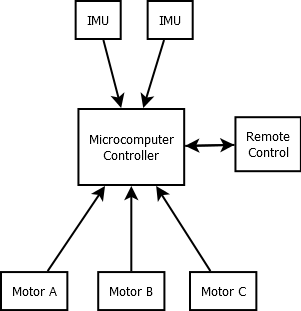
\includegraphics[width=.5\textwidth]{Images/Block-Diagram}
			\caption{Block diagram showing the relationships between each component of \BBB}
			\label{fig: Overview}
		\end{figure}
		
		\subsection{General}
		This specification establishes the design, construction, performance, development, and test requirements for the \BBB system. These requirements represent an effort to meet the aforementioned goals.
		
		\subsection{Acronyms}
		\begin{itemize}
			\item \textbf{\BBB} - Ball Balancing Bot.
			\item \textbf{IMU} - Inertial Measurement Unit.
		\end{itemize}
		\subsection{Definitions}
		\begin{itemize}
			\item \textbf{Remote Control} - An human interface to send input commands to the robot from a distance of 2-10 feet.
		\end{itemize}
		
		%\pagebreak	
		%\section{Applicable Documents}
		%The following documents shown shall form part of the specifications for this project. In the event of a conflict between requirements, priority shall first go to the contract, second to this document, and lastly to these reference documents.
		%\subsection{Industry Documents}
		%\begin{enumerate}
		%	\item Z-Wave
		%\end{enumerate}
		
		\pagebreak
		\section{Stakeholder Requirements}
		The stakeholders for the complete \BBB system are:
		\begin{enumerate}
			\item Developers
			\item Utah State university Electrical Engineering department
			\item Dr. Don Cripps
			\item Professor Taylor Peterson
			\item Customers/Users
		\end{enumerate}
		
		\subsection{Stakeholder User Stories}
		The primary stakeholders needs are described below.
		\begin{enumerate}
			\item \BBB must use some type of feedback control system.\\
			\vspace{1em}
			\underline{User Story}\\
			As a student in Dr. Cripp's Mechatronics class, I must use a feedback system to control motors, actuators, etc in this project.
			
			\item \BBB must use some type of microcomputer for control of the system.	\\	
			\vspace{1em}
			\underline{User Story}\\
			As a student in Taylor Peterson's Microcomputer Interfacing class, I must use some type of microcomputer or embedded system in the project.
			
			\item \BBB must be remote controllable to navigate about a room.\\
			\vspace{1em}
			\underline{User Story}\\
			As this project will be used to count towards two separate classes, some additional degree of difficulty must be added into the project. As a robot that balances atop a ball is cool, it'd be much better if you could drive it around.
			
			\item \BBB must balance atop a standard sports ball.\\
			\vspace{1em}
			\underline{User Story}\\
			As a user, I want to be able to put the robot on something like a basketball, soccer ball, or even a volleyball. That way I don't have to have a specialized ball just for \BBB.			
		\end{enumerate}
		
		\pagebreak
		\section{Engineering Requirements}
			\subsection{Interface Requirements}
				\subsubsection{} The robot shall fit atop a basketball, soccer ball, or volley ball.
				\subsubsection{} The robot shall be controllable via remote input from the user.
			\subsection{Functional Requirements}
				\subsubsection{} The robot shall make use of a feedback control system.
				\subsubsection{} The robot shall make use of a microcomputer or embedded system..
				\subsubsection{} The robot shall balance on top of a ball.
				\subsubsection{} The robot shall be drivable from remote control input.
			\subsection{Functional Support Requirements}
				\subsubsection{} The robot shall move in any horizontal direction.
				\subsubsection{} The robot shall be able to withstand a one-foot drop on it's side.
		
		\pagebreak		
		\section{Verification of Requirements}
			\subsection{Interface Requirements Verification}
				\subsubsection{} Does the robot sit atop a basketball, soccer ball, or volley ball?
				\subsubsection{} Can the robot be directed via remote control?
			\subsection{Functional Requirements Verification}
				\subsubsection{} Does the robot use a feedback control system?
				\subsubsection{} Does the robot use a a microcomputer or an embedded system?
				\subsubsection{} Does the robot balance on top of a ball?
				\subsubsection{} Can the robot be driven from remote control?
			\subsection{Functional Support Requirements Verification}
				\subsubsection{} Can the robot move in any horizontal direction?
				\subsubsection{} Can the robot be dropped from one foot onto it's side and not break?
		
	\end{flushleft}
\end{document}
